\chapter{ Simulations and Results }\label{simulationsAndResults}

In the simulations the following mixture of normal distributions was used for $\pi$'s density:

\begin{equation}\label{experimental pi}
f(x) = 
\sum_{i=1}^{20} \frac{\omega_i}{ \sigma_i \sqrt{2 \pi} } \exp \Big( -\frac{(x - \mu_i)^\tran (x - \mu_i)}{2 \sigma_i^2} \Big),	
\end{equation}
where $\sigma_1 = \dots = \sigma_{20} = 0.1$, $\omega_1 = \dots = \omega_{20} = 0.05 $ and the means $\mu_i$ are given by

\begin{table}[ht]
	\centering
\begin{tabular}{rrrrrrrrrr}
  \hline
1 & 2 & 3 & 4 & 5 & 6 & 7 & 8 & 9 & 10 \\ 
  \hline
2.18 & 8.67 & 4.24 & 8.41 & 3.93 & 3.25 & 1.70 & 4.59 & 6.91 & 6.87 \\ 
  5.76 & 9.59 & 8.48 & 1.68 & 8.82 & 3.47 & 0.50 & 5.60 & 5.81 & 5.40 \\ 
   \hline
\end{tabular}
\end{table}
and 

\begin{table}[ht]
	\centering
\begin{tabular}{rrrrrrrrrr}
  \hline
11 & 12 & 13 & 14 & 15 & 16 & 17 & 18 & 19 & 20 \\ 
  \hline
5.41 & 2.70 & 4.98 & 1.14 & 8.33 & 4.93 & 1.83 & 2.26 & 5.54 & 1.69 \\ 
  2.65 & 7.88 & 3.70 & 2.39 & 9.50 & 1.50 & 0.09 & 0.31 & 6.86 & 8.11 \\ 
   \hline
\end{tabular}
\end{table}
 
Figure \ref{ToyExample} inspects visually the density. One notices easily that different peaks get intermingled, as only $15$ out of $20$ peaks are visible.  

\begin{figure}
	\begin{minipage}[b]{.5\linewidth}
		\centering 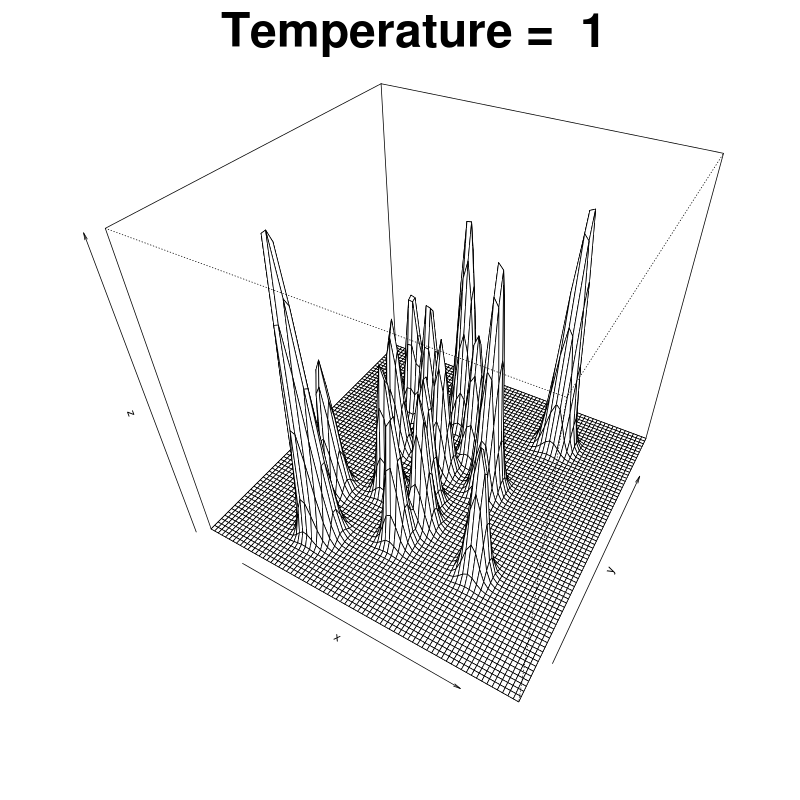
\includegraphics[scale=.25]{./img/Liang_perspective.png}
		\subcaption{Perspective view}\label{LiangContour}
	\end{minipage}%
	\begin{minipage}[b]{.5\linewidth}
		\centering 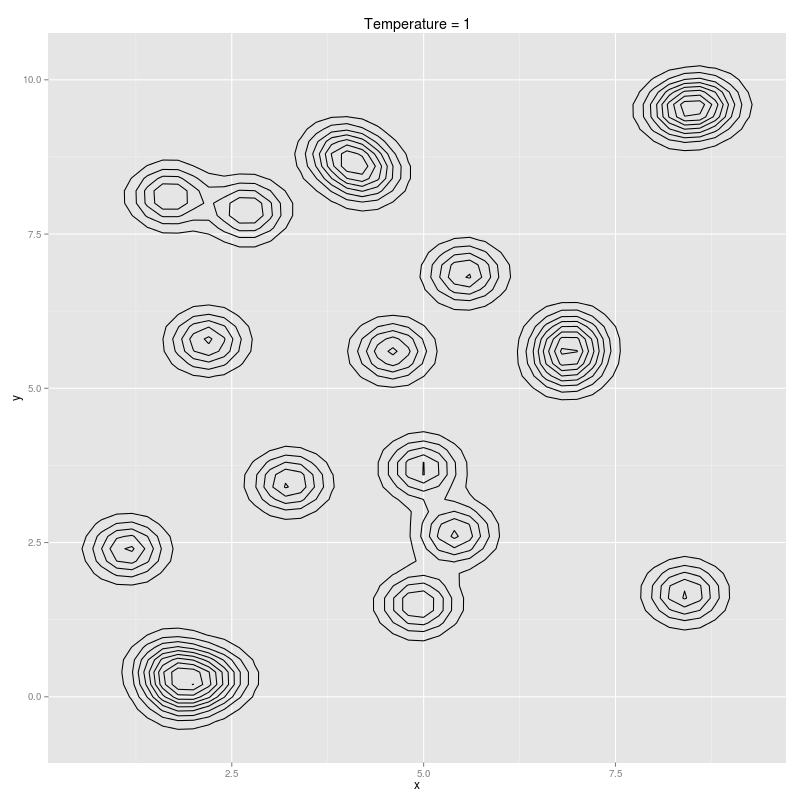
\includegraphics[scale=.25]{./img/Liang_Contour_plot.png}
	\subcaption{Level-set view}\label{LiangPerspective}
	\end{minipage}
	\caption{Toy-example density.}\label{ToyExample}
\end{figure}

